\pagestyle{fancy}
\chapterA{Modelado hardware con VHDL. Introducción a las FPGAs}
\section{Flujo de diseño}

TODO

\section{Lenguaje de descripción hardware}
\gls{hdl} es un lenguaje específicamente creado para el diseño de circuitos, tanto a nivel de puerta como a nivel e comportamiento. La estructura del lenguaje sugiere el diseño hardware.

Los \gls{hdl} se usan para poder descubrir problemas en el diseño del hardware antes de su implementación física. Como la complejidad de los sistemas electrónicos crece exponencialmente, es necesaria una herramienta que trabaje con el ordenador. Por último, gracias a estas herramientas más de una persona puede trabajar en el mismo proyecto

En este curso usaremos \gls{vhdl}, esto nos permite hacer descripciones de la estructura del circuito con:
\begin{itemize}
	\item Descomposición en sub-circuitos
	\item Interconexión de sub-circuitos
	\item comportamiento
	\item Estructural
\end{itemize}
También permite la especificación de un circuito utilizando formas familiares de lenguajes de programación y la simulación del circuito antes de su fabricación.

Un \gls{hdl} tiene que ser capaz de simular el comportamiento real del hardware sin que el programador necesite imponer restricciones.

\noindent \textbf{Ejemplo 1:}

\begin{table}[H]
	\centering
	\begin{tabular}{|l|l|}
		\hline
		\cellcolor[HTML]{70A9FC} t = 5ns & \cellcolor[HTML]{70A9FC} t=10ns \\ \hline
		A = 0                            & A = 1                           \\ \hline
		B = 1                            & B = 1                           \\ \hline
		C = 0                            & C = 0                           \\ \hline
	\end{tabular}
\end{table}

\begin{multicols}{2}
	\underline{Descripción 1:}

	D = A and B;

	S = D or C;

	\columnbreak

	\underline{Descripción 2:}

	S = D or C;

	D = A and B;
\end{multicols}

\textcolor{cyan}{?`Se obtiene el mismo resultado?} No, en la descripción 1 en t = 10ns el valor de S será 1, mientras que en la descripción 2 seguirá siendo 0.


\newpage
\section{Simulación con VHDL}
\gls{vhdl} realiza la simulación siguiendo la técnica de \textbf{simulación por eventos discretos}, esto permite avanzar el tiempo a intervalos variables, en función de la planificación de ocurrencia de eventos.
La simulación consta de tres fases:
\begin{itemize}
	\item\textbf{Fase 0: }fase de inicialización donde las señales se les asignan unos valores iniciales y se pone el tiempo a cero. La asignación se hace rellenando una lista de eventos para el instante t = 0.
	\item\textbf{Fase 1: }todas las transiciones planificadas para ese tiempo se ejecutan
	\item\textbf{Fase 2: }las señales que se han modificado en consecuencia de las transiciones planificadas en el instante t se escriben en la lista de eventos planificándose para el instante t + $\delta$, donde $\delta$ es un instante infinitesimal. Una vez acabado esta fase se vuelve a la fase 1 hasta que se termine la simulación.
\end{itemize}

\begin{multicols}{3}
	\begin{figure}[H]
		\centering
		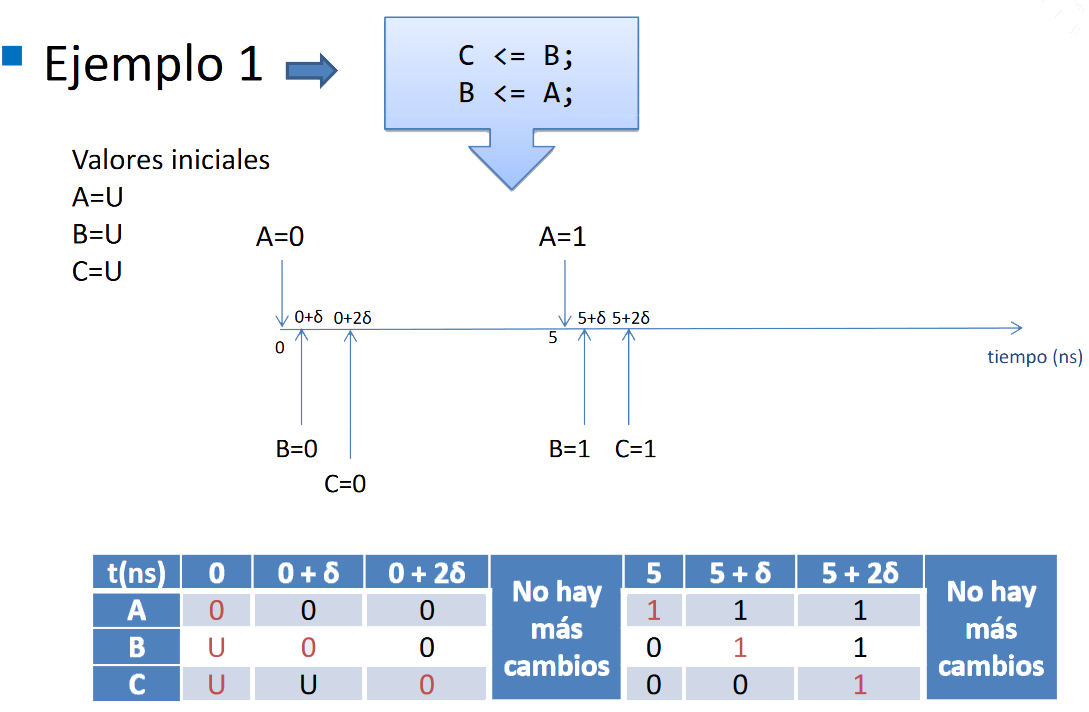
\includegraphics[width=0.3\textwidth]{images/Tema_1/VHDL_Ejemplo_1.PNG}
	\end{figure}
	\vfill
	\begin{figure}[H]
		\centering
		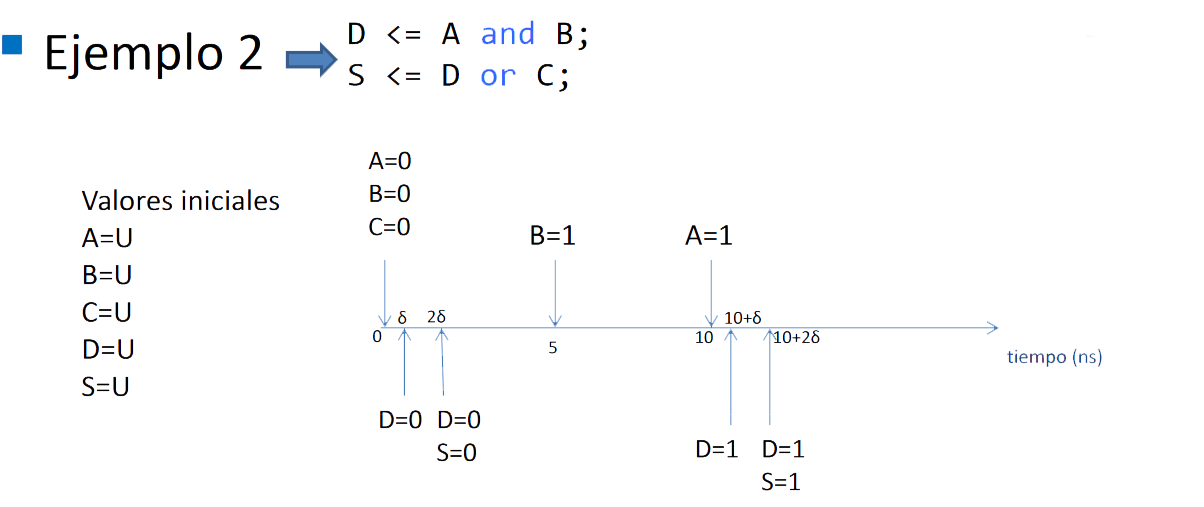
\includegraphics[width=0.3\textwidth]{images/Tema_1/VHDL_Ejemplo_2.PNG}
	\end{figure}
	\vfill
	\begin{figure}[H]
		\centering
		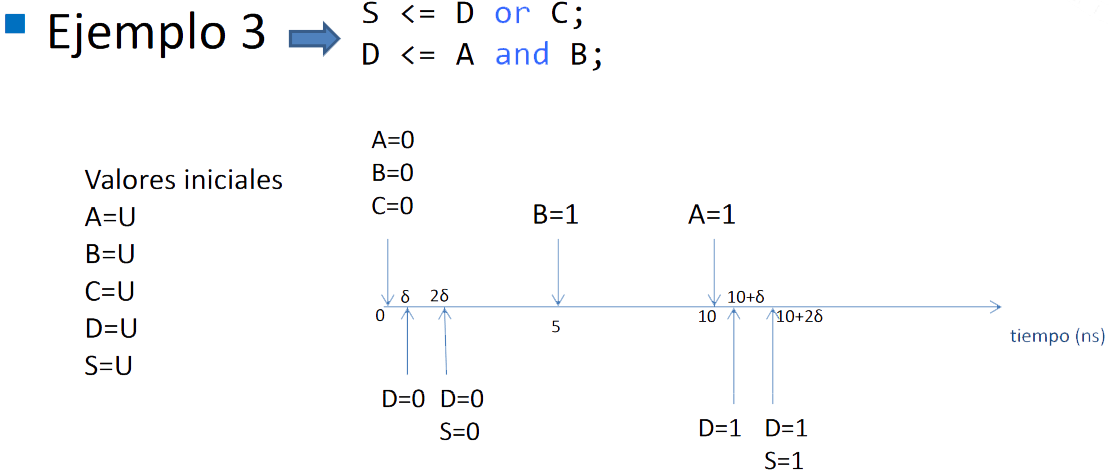
\includegraphics[width=0.3\textwidth]{images/Tema_1/VHDL_Ejemplo_3.PNG}
	\end{figure}
\end{multicols}


\textbf{Pregunta ejemplo 3: }?`Qué pasaría si en 5 en vez de cambiar B cambia C? S=1 ya que D or C si c = 1 siempre es 1.


\section{Estructura de un modelo VHDL}
Un sistema digital está descrito por sus entradas y sus salidas, donde las salidas dependen de las entradas.
Los modelos \gls{vhdl} están formados por dos partes:
\begin{multicols}{2}
	\begin{figure}[H]
		\centering
		\lstinputlisting[style=customVHDL]{Code/Tema_1/Ejemplo_Entity_1.vhd}
		\caption{Ejemplo Entity}
	\end{figure}
	\vfill
	\begin{figure}[H]
		\centering
		\lstinputlisting[style=customVHDL]{Code/Tema_1/Ejemplo_Architecture_1.vhd}
		\caption{Ejemplo Architecture}
	\end{figure}
\end{multicols}

La entity define externamente el circuito o subcircuito,  especifica el nombre y el número de puertos, su tipo de datos y si son de entrada o salida, tiene toda la información necesaria para conectar tu circuito a otros circuitos.
La architecture define internamente el circuito, sus señales internas, funciones, procedimientos, constantes, etc.


Cada architecture va asociada a una entity y se indica en la primera sentencia. Antes del begin se definen las señales, los tipos y los componentes

\begin{figure}[H]
	\centering
	\lstinputlisting[style=customVHDL]{Code/Tema_1/Ejemplo_completo_1.vhd}
	\caption{Ejemplo Entity y Architecture}
\end{figure}

\section{Elementos básicos de VHDL}

Las sentencias concurrentes siempre se encuentran fuera de los PROCESS, aparecen en cualquier punto del programa después del begin de la arquitectura,  es lógica combinacional pura y siempre tiene un ELSE final o un WHEN OTHERS.

\begin{multicols}{2}
	\begin{figure}[H]
		\centering
		\lstinputlisting[style=customVHDL]{Code/Tema_1/Ejemplo_When-Else.vhd}
		\caption{Ejemplo When-Else}
	\end{figure}
	\vfill
	\begin{figure}[H]
		\centering
		\lstinputlisting[style=customVHDL]{Code/Tema_1/Ejemplo_When-Select-Else.vhd}
		\caption{Ejemplo With-Select-Else}
	\end{figure}
\end{multicols}


Los procesos son sentencias concurrentes. Solo se ejecutan esas sentencias que se encuentran dentro del proceso si alguna de las señales de la lista de sensibilidad ha cambiado de valor. La lista de sensibilidad es opcional, si no existe el proceso se ejecuta infinitas veces. Es un código secuencial.
\begin{figure}[H]
	\centering
	\lstinputlisting[style=customVHDL, xleftmargin=.2\textwidth, xrightmargin=.2\textwidth]{Code/Tema_1/Ejemplo_Process.vhd}
	\caption{Ejemplo Process}
\end{figure}

Las secuencias condicionales van dentro de un process, si la lista de sensibilidad está incompleta, el comportamiento del process será incorrecto. Estas sentencias deben tener un caso por defecto.
\begin{multicols}{2}
	\begin{figure}[H]
		\centering
		\lstinputlisting[style=customVHDL]{Code/Tema_1/Ejemplo_If-Then-Else.vhd}
		\caption{Ejemplo If-Then-Else}
	\end{figure}
	\vfill
	\begin{figure}[H]
		\centering
		\lstinputlisting[style=customVHDL]{Code/Tema_1/Ejemplo_Case.vhd}
		\caption{Ejemplo Case}
	\end{figure}
\end{multicols}

Ejemplos de bucles en VHDL:
\begin{multicols}{3}
	\begin{figure}[H]
		\centering
		\lstinputlisting[style=customVHDL]{Code/Tema_1/Ejemplo_Loop_1.vhd}
		\caption{Loop simple}
	\end{figure}
	\vfill
	\begin{figure}[H]
		\centering
		\lstinputlisting[style=customVHDL]{Code/Tema_1/Ejemplo_For_Loop.vhd}
		\caption{For Loop}
	\end{figure}
	\vfill
	\begin{figure}[H]
		\centering
		\lstinputlisting[style=customVHDL]{Code/Tema_1/Ejemplo_While_Loop.vhd}
		\caption{While Loop}
	\end{figure}
\end{multicols}

Las sentencias wait se usan en procesos, procedimientos y funciones y, como indica su nombre, hace que haya un tiempo de espera. Puede ser de tres tipos:
\begin{itemize}
	\item\textbf{wait for} <timeout clause, time delay>: \textcolor{magenta}{wait for} 10 ns;
	\item\textbf{wait until} <condition>: \textcolor{magenta}{wait until} clk = '1';
	\item\textbf{wait on} <sensitive clause, event>: \textcolor{magenta}{wait on} in1;
\end{itemize}


Atributos:
\begin{itemize}
	\item S'\textbf{DELAYED}(t) es el valor de la señal S en el tiempo actual -t.
	\item S'\textbf{STABLE} es true si no hay ningún evento ocurriendo para S.
	\item S'\textbf{STABLE}(t) es true si no hay eventos ocurriendo en S durante t unidades de tiempo.
	\item S'\textbf{QUIET} es true si no hay eventos en ese ciclo de simulación para la señal S.
	\item S'\textbf{QUIET}(t) es true si no hay eventos en ese ciclo de simulación para la señal S durante t unidades de tiempo.
	\item S'\textbf{TRANSACTION} es un valor BIT, el inverso del valor previo de cada ciclo en que S está activo.
	\item S'\textbf{EVENT} es true si S tiene un evento en el ciclo de simulación.
	\item S'\textbf{ACTIVE} es true si S está activa durante el ciclo de simulación.
	\item S'\textbf{LAST\_EVENT} es el tiempo desde el último evento en S.
	\item S'\textbf{LAST\_ACTIVE} es el tiempo desde la última vez que S estuvo activa.
	\item S'\textbf{LAST\_VALUE} es el valor anterior de S.
\end{itemize}

Tipos de datos:
\begin{itemize}
	\item Tipos enteros y reales:
	      \begin{itemize}
		      \item INTEGER
		      \item NATURAL
		      \item REAL
	      \end{itemize}
	\item Tipos físicos
	      \begin{itemize}
		      \item TIME
		      \item RESISTANCE
	      \end{itemize}
	\item Tipos enumerados: conjuntos de posibles valores
	      \begin{itemize}
		      \item BIT {0,1}
		      \item BOOLEAN {TRUE, FALSE}
		      \item CHARACTER {ASCII CHARACTERS}
		      \item STD\_LOGIC {U, X, 0, 1, Z, W, L, H, -}
	      \end{itemize}
\end{itemize}

Se pueden definir tipos personalizados

\begin{figure}[H]
	\centering
	\lstinputlisting[style=customVHDL]{Code/Tema_1/Ejemplo_Tipos_Personalizados.vhd}
	\caption{Ejemplo tipos personalizados}
\end{figure}

Arrays:

\begin{figure}[H]
	\centering
	\lstinputlisting[style=customVHDL]{Code/Tema_1/Ejemplo_Arrays.vhd}
	\caption{Ejemplo Arrays}
\end{figure}

Un \textbf{componente} es una entidad que se describe dentro de una arquitectura
\begin{figure}[H]
	\centering
	\lstinputlisting[style=customVHDL, xleftmargin=.2\textwidth, xrightmargin=.2\textwidth]{Code/Tema_1/Ejemplo_Component.vhd}
	\caption{Ejemplo Component}
\end{figure}


\textbf{Generate:} las secuencias de generación de componentes permiten crear una o más copias de un conjunto de interconexiones, lo cual facilita el diseño de circuitos mediante descripciones estructurales

\begin{figure}[H]
	\centering
	\lstinputlisting[style=customVHDL, xleftmargin=.2\textwidth, xrightmargin=.2\textwidth]{Code/Tema_1/Ejemplo_Generate.vhd}
	\caption{Ejemplo Generate}
\end{figure}

Un \textbf{paquete} son agrupaciones de tipos, funciones y procedimientos personalizados. Pueden ser incluidos en uno o varios diseños, normalmente se definen en ficheros .vhd dedicados.

\begin{figure}[H]
	\centering
	\lstinputlisting[style=customVHDL, xleftmargin=.2\textwidth, xrightmargin=.2\textwidth]{Code/Tema_1/Ejemplo_Package.vhd}
	\caption{Ejemplo Package}
\end{figure}

\section{Entidades parametrizables}
Una entity puede tener una lista de parámetros. El valor por defecto de los parámetros genéricos es opcional, sin embargo, no se puede sintetizar un diseño con parámetros que no tengan asignado un valor.

Al instanciar este componente en otro fichero, hay que asignar un valor a n si y solo si no se le dio un valor por defecto en su declaración de entity.

Se  puede  utilizar  la  asignación (others=> ‘0’) o (others=> ‘1’) para asignar el valor “0...0” o “1...1” a una señal de longitud parametrizable.

\section{Testbench de simulación}
Para conocer si nuestro diseño funciona correctamente tendremos que introducir unos estímulos en las entradas y comprobar que las salidas obtenidas son las deseadas.

\textbf{Estructura básica:}
\begin{enumerate}
	\item Se crea una entidad de simulación sin puertos de entrada ni de salida
	\item Se añade como component la entity a verificar
	\item Se definen tantas señales como puertos de la entity del diseño a verificar
	\item Se instancia el component igualando las señales internas a las entradas
	\item Se crea el process de simulación, no tiene lista de sensibilidad
	\item Se definen los valores iniciales de las entradas
	\item Se definen los valores de las entradas en los siguientes instantes de tiempo
\end{enumerate}

Cómo implementar una entrada periódica: clk
\begin{figure}[H]
	\centering
	\lstinputlisting[style=customVHDL, xleftmargin=.2\textwidth, xrightmargin=.2\textwidth]{Code/Tema_1/Ejemplo_Clk.vhd}
	\caption{Ejemplo Clk}
\end{figure}

Como este process no acaba con un wait sin for, se repetirá indefinidamente.


\section{Introducción a las FPGAs}
Una FPGA es un hardware de prototipado automático. Inicialmente servía para lo mismo que un entrenador, con la diferencia de que el circuito se implementaba automáticamente. Debido a su gran capacidad de procesamiento, versatilidad y a las herramientas de diseño 9. Introducción a las TC versatilidad y a las herramientas de diseño disponibles, actualmente existen circuitos comerciales que llevan FPGAs incorporadas.

Los componentes de una FPGA son:
\begin{itemize}
	\item Celdas de entrada salida
	\item Celdas lógicas programables
	\item Celdas de interconexión programables (las estructuras de interconexionado son muy costosas)
	\item Memorias(opcional)
	\item Multiplicadores(opcional)
	\item Micro-controladores(opcional)
\end{itemize}

Una CLB contiene:
\begin{itemize}
	\item Look-Up Tables: son memorias \gls{rom} que almacenan 1x16 bits, pueden implementar cualquier función lógica de 4 entradas.
	\item Biestables: se utilizan en el caso de que la celda deba implementar HW secuencial. Se pueden configurar si son disparados por flanco o por nivel.
	\item Multiplexores: para interconectar las entradas con los módulos o los módulos entre si se utilizan multiplexores
\end{itemize}
